\documentclass{article}[18pt]
\ProvidesPackage{format}
%Page setup
\usepackage[utf8]{inputenc}
\usepackage[margin=0.7in]{geometry}
\usepackage{parselines} 
\usepackage[english]{babel}
\usepackage{fancyhdr}
\usepackage{titlesec}
\hyphenpenalty=10000

\pagestyle{fancy}
\fancyhf{}
\rhead{Sam Robbins}
\rfoot{Page \thepage}

%Characters
\usepackage{amsmath}
\usepackage{amssymb}
\usepackage{gensymb}
\newcommand{\R}{\mathbb{R}}

%Diagrams
\usepackage{pgfplots}
\usepackage{graphicx}
\usepackage{tabularx}
\usepackage{relsize}
\pgfplotsset{width=10cm,compat=1.9}
\usepackage{float}

%Length Setting
\titlespacing\section{0pt}{14pt plus 4pt minus 2pt}{0pt plus 2pt minus 2pt}
\newlength\tindent
\setlength{\tindent}{\parindent}
\setlength{\parindent}{0pt}
\renewcommand{\indent}{\hspace*{\tindent}}

%Programming Font
\usepackage{courier}
\usepackage{listings}
\usepackage{pxfonts}

%Lists
\usepackage{enumerate}
\usepackage{enumitem}

% Networks Macro
\usepackage{tikz}


% Commands for files converted using pandoc
\providecommand{\tightlist}{%
	\setlength{\itemsep}{0pt}\setlength{\parskip}{0pt}}
\usepackage{hyperref}

% Get nice commands for floor and ceil
\usepackage{mathtools}
\DeclarePairedDelimiter{\ceil}{\lceil}{\rceil}
\DeclarePairedDelimiter{\floor}{\lfloor}{\rfloor}

% Allow itemize to go up to 20 levels deep (just change the number if you need more you madman)
\usepackage{enumitem}
\setlistdepth{20}
\renewlist{itemize}{itemize}{20}

% initially, use dots for all levels
\setlist[itemize]{label=$\cdot$}

% customize the first 3 levels
\setlist[itemize,1]{label=\textbullet}
\setlist[itemize,2]{label=--}
\setlist[itemize,3]{label=*}

% Definition and Important Stuff
% Important stuff
\usepackage[framemethod=TikZ]{mdframed}

\newcounter{theo}[section]\setcounter{theo}{0}
\renewcommand{\thetheo}{\arabic{section}.\arabic{theo}}
\newenvironment{important}[1][]{%
	\refstepcounter{theo}%
	\ifstrempty{#1}%
	{\mdfsetup{%
			frametitle={%
				\tikz[baseline=(current bounding box.east),outer sep=0pt]
				\node[anchor=east,rectangle,fill=red!50]
				{\strut Important};}}
	}%
	{\mdfsetup{%
			frametitle={%
				\tikz[baseline=(current bounding box.east),outer sep=0pt]
				\node[anchor=east,rectangle,fill=red!50]
				{\strut Important:~#1};}}%
	}%
	\mdfsetup{innertopmargin=10pt,linecolor=red!50,%
		linewidth=2pt,topline=true,%
		frametitleaboveskip=\dimexpr-\ht\strutbox\relax
	}
	\begin{mdframed}[]\relax%
		\centering
		}{\end{mdframed}}



\newcounter{lem}[section]\setcounter{lem}{0}
\renewcommand{\thelem}{\arabic{section}.\arabic{lem}}
\newenvironment{defin}[1][]{%
	\refstepcounter{lem}%
	\ifstrempty{#1}%
	{\mdfsetup{%
			frametitle={%
				\tikz[baseline=(current bounding box.east),outer sep=0pt]
				\node[anchor=east,rectangle,fill=blue!20]
				{\strut Definition};}}
	}%
	{\mdfsetup{%
			frametitle={%
				\tikz[baseline=(current bounding box.east),outer sep=0pt]
				\node[anchor=east,rectangle,fill=blue!20]
				{\strut Definition:~#1};}}%
	}%
	\mdfsetup{innertopmargin=10pt,linecolor=blue!20,%
		linewidth=2pt,topline=true,%
		frametitleaboveskip=\dimexpr-\ht\strutbox\relax
	}
	\begin{mdframed}[]\relax%
		\centering
		}{\end{mdframed}}
\lhead{CSys}
\usepackage{karnaugh-map}

\begin{document}
\begin{center}
\underline{\huge Digital Electronics and Machine Architecture}
\end{center}
\section{Introduction}
\subsection{von Neumann Architecture}
\begin{itemize}
	\item Memory holds both programs and data
	\item Memory is addressed linearly
	\item Memory is addressed by location, the contents are irrelevant
	\item Instructions executed sequentially, unless a branch or reset occurs
\end{itemize}
\subsection{Harvard Architecture}
This has separate memory for instructions and data
\begin{itemize}
	\item Quicker to execute as can access instruction and data at the same time
	\item Simpler to follow/analyze code
	\item Avoids the potential for some malware/bugs due to self modifying code
\end{itemize}
\section{CPU Architecture}
\subsection{Components of a CPU}
\begin{itemize}
	\item Memory - RAM
	\item Registers - Special memory locations that can be accessed very fast
	\item ALU
	\item Buses - Wires that carry data between components
	\item Control Unit - Responsible for directing the flow of instructions and data within the CPU
\end{itemize}
\subsection{Registers}
Manipulated directly by the Control Unit\\
Size of registers can vary from 1 to 128 bits\\
\\
\textbf{Accumulator} - considered part of the ALU, has general purpose registers for
\begin{itemize}
	\item Holding data
	\item Holding interim and final results of arithmetic operations
	\item Holding data waiting to be transferred between different memory locations
	\item Holding data waiting to be transferred between different memory locations
	\item Holding data waiting to be transferred between I/O and memory
\end{itemize}
Program counter - Holds the address of the next instruction to be executed\\
Instruction Register - Holds the actual instruction being executed\\
Flags - 1 bit registers used to keep track of special conditions\\
\\
Memory Address Register - Holds the address of a memory location to be accessed\\
Memory Data Register - Holds the value that is being stored to or retrieved from the memory location currently addressed by the MAR
\subsection{Buses}
Buses are used to:
\begin{itemize}
	\item Transfer data between the different points on the CPU
	\item Transfer data between the CPU and main memory
	\item Transfer data between computer peripherals and the CPU
\end{itemize} 
A bus is a group of electrical conductors (lines) used to carry signal, they have 4 general categories
\begin{itemize}
	\item Data
	\item Address
	\item Control
	\item Power
\end{itemize}
\textbf{Point to point} - Bus carries the signal from a specific source to a specific destination\\
\textbf{Broadcast} - Bus used to carry signals to many devices\\
\textbf{Bus interface bridges} - Allow communications between the different buses
\section{Binary}
\begin{itemize}
	\item Nibble - 4 Bits
	\item Byte - 8 Bits
	\item Half Word - 16 Bits
	\item Word - 32 bits
	\item Double word - 64 bits
\end{itemize}
\subsection{Decimal fractions to binary}
\begin{itemize}
	\item Repeatedly multiply the number by 2, until the fractional part is 0
	\item If the ith result is greater than or equal to 1, places 1 in the ith position to the right of the radix, retain only fractional part
	\item Else, place a 0 in the ith position to the right of the radix
\end{itemize}
\section{Binary Arithmetic and Floating Point}
\subsection{Negative numbers}
\textbf{One's complement}
\begin{itemize}
	\item The negative of a number is represented by flipping each bit
	\item Higher order bit indicates the sign of the number
\end{itemize}
\textbf{Twos complement}
\begin{itemize}
	\item A negative number is obtained by flipping each bit and adding 1
	\item Higher order bit indicates sign of number
	\item One representation for 0
\end{itemize}
\textbf{Add a bias}
\begin{itemize}
	\item For k bit numbers, add a bias of $2^{k+1}$, then store in normal binary
	\item Can store numbers between $-(2^{k-1}-1)$ and $2^{k-1}$
	\item The higher order bit does not indicate the sign of the number
\end{itemize}
\subsection{Floating point representation}
Floating point representation has three fields
\begin{itemize}
	\item Sign bit S
	\begin{itemize}
		\item 0 indicates positive, 1 indicates negative
	\end{itemize}
	\item Exponent e
	\begin{itemize}
		\item Stored with a bias of 127
		\item 0 and 255 have special meanings
		\begin{itemize}
			\item Exponent 0 with mantissa 0 gives the number 0
			\item Exponent 0 with non zero mantissa - "subnormal numbers"
			\item Exponent 255 with mantissa 0 gives + or - infinity
			\item Exponent 255 with non zero mantissa: not a number
		\end{itemize}
	\end{itemize}
	\item Mantissa M
	\begin{itemize}
		\item Binary number
		\item Always scaled so that the radix point is after the leading 1
	\end{itemize}
\end{itemize}
\section{Logic Gates and Transistors}
\subsection{Transistors}
\begin{center}
	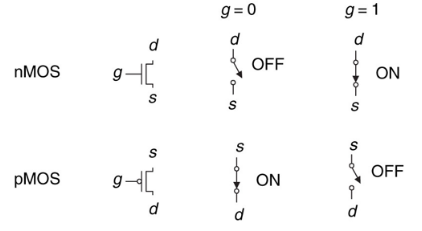
\includegraphics[scale=0.7]{transistors}
\end{center}
The most common transistor is the MOSFET\\
Silicon is a poor conductor of electricity: all the available electrons are used to form bonds with neighbouring atoms.\\
Impurities (dopants) provide extra electrons or electron holes which increase conductivity.\\
Diode
\begin{center}
	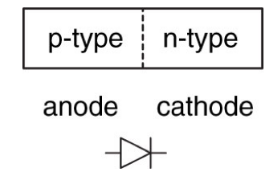
\includegraphics[scale=0.7]{diode}
\end{center}
Capacitor - Two pieces of conductive material separated by an insulator\\
\\
nMOS transistor
\begin{center}
	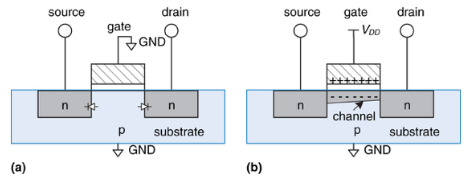
\includegraphics[scale=0.7]{nMOS}
\end{center}
pMOS transistor
\begin{center}
	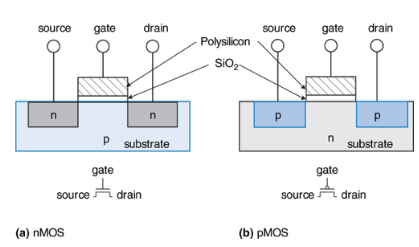
\includegraphics[scale=0.7]{pMOS}
\end{center}
\subsection{Supply voltage}
The \textbf{low} voltage of the system is 0V\\
Historically the high voltage was 5V, called $V_{DD}$. However modern chips have moved to lower voltages to save power and avoid overloading transistors.\\
The mapping of the continuous voltage at any point between 0 and 1 is governed by defining logic levels
\subsection{Logic levels}
\begin{center}
	\includegraphics[scale=0.7]{"Logic Levels"}
\end{center}
\textbf{Output range}
\begin{itemize}
	\item $V_{OH}$ - Output High
	\item $V_{OL}$ - Input Low
\end{itemize}
\textbf{Noise Margins}
\begin{itemize}
	\item $NM_H$ - Noise Margin High
	\item $NM_L$ - Noise Margin Low
\end{itemize}
\textbf{Input range}
\begin{itemize}
	\item $V_{IH}$ - Input High
	\item $V_{IL}$ - Input Low
\end{itemize}
\subsection{Transfer Characteristics}
\begin{center}
	\includegraphics[scale=0.7]{"Transfer Characteristics"}
\end{center}
An \textbf{ideal inverter} would output $V_{DD}$ for inputs up to $V_{DD}/2$ and 0 otherwise\\
However real circuits are not ideal
\subsection{The Statistic Discipline}
You can only allow circuit elements that all satisfy the same logic levels
\section{Boolean Algebra}
\subsection{Functionally Complete Sets}
AND, OR and NOT form a functionally complete set as all propositional logic can be formed from them. It is easiest to prove that other sets are functionally complete by proving that they can form those sets.\\
For example, it can be shown that NOR is functionally complete
\begin{center}
	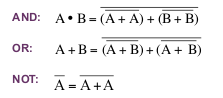
\includegraphics[scale=0.7]{NOR}
\end{center}
NAND can also be shown to be functionally complete and uses less silicon for the same performance so are used as universal gates
\subsection{Circuits}
A circuit has
\begin{itemize}
	\item One or more discrete valued input terminals
	\item One or more discrete valued output terminals
	\item A specification of the relationship between inputs and outputs
	\item A specification of the delay between inputs changing and outputs responding
\end{itemize}
A circuit is made up of elements and nodes
\begin{itemize}
	\item \textbf{Element} - A subcircuit
	\item \textbf{Node} - A wire joining elements
\end{itemize}
\subsection{Combinational Logic}
Rules:
\begin{itemize}
	\item Individual gates are combinational circuits
	\item Every circuit element must be a combinational circuit
	\item Every node is either an input to the circuit or connecting to exactly one output of a circuit element
	\item The circuit has no cyclic paths - every path through the circuit visits any node at most once
\end{itemize}
\subsection{Boolean Algebra}
\begin{itemize}
	\item Complement/Inverse - $\overline{A}$
	\item Product/Implicant - $A\cdot B$
	\item Minterm - Product involving all inputs to a function
	\item Sum/Implicant (Yeah, they're both called implicant) - $A+B$
	\item Maxterm - A sum involving all inputs to a function
\end{itemize}
As you know from MCS all boolean expressions can be written in sum of product or product of sum form (DNF or CNF)
\subsection{Axioms of Boolean Algebra}
\begin{center}
	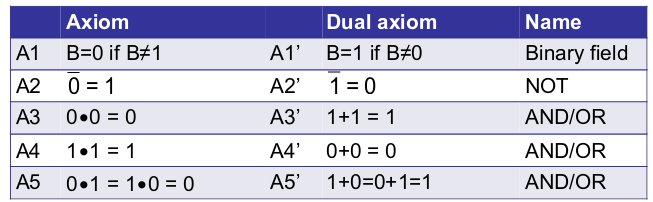
\includegraphics[scale=0.7]{Axioms}
\end{center}
\begin{center}
	\includegraphics[scale=0.7]{"Theorems of One Variable"}
\end{center}
\section{Karnaugh Maps}
Boolean expressions can be simplified by spotting terms of the form $PA+P\overline{A}$ (resolution)\\
Neighbouring 1s in the K-Map are of the form $PA+P\overline{A}$ (note that the numbers ascend with 1 bit difference rather than numerically)\\
\begin{karnaugh-map}*[4][2][1][AB][C]
	\minterms{0,4}
	\autoterms[0]
	\implicant{0}{4}
\end{karnaugh-map}\\
Forming a Karnaugh Map
\begin{enumerate}
	\item Create a map so that neighbouring terms differ in the negation of one variable
	\item Circle all rectangular blocks of ones in the map using as few circles as possible
	\item Each circle must be a power of 2 in each dimension
	\item Read off the implicants that were circled (what formula defines that circle)
\end{enumerate}
\section{Circuits}
\subsection{Key Circuits}
Combinatorial circuits (Output depends only on current input)
\begin{itemize}
	\item Adders - Add the contents of two registers
	\item Decoders - Use a binary number to activate a single line
	\item Multiplexors - Use a binary number to select an input
\end{itemize}
Sequential circuits (Output depends on state and input)
\begin{itemize}
	\item Latches/Flip Flops - Basic memory element
\end{itemize}
\subsection{Half Adder}
This has a truth table that follows the basic binary addition rules for 1 bit numbers
\begin{center}
	\includegraphics[scale=0.7]{"Half Adder"}
\end{center}
A full adder also takes into account the carry from the previous bit, allowing them to be chained to add any length of number
\begin{center}
	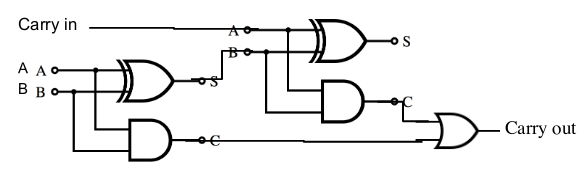
\includegraphics[scale=0.7]{Adder}
\end{center}
They can be chained like so:
\begin{center}
	\includegraphics[scale=0.7]{"Chaining Adders"}
\end{center}
\subsection{Subtractor}
By creating twos complement negative we can subtract two numbers, with the circuit below
\begin{center}
	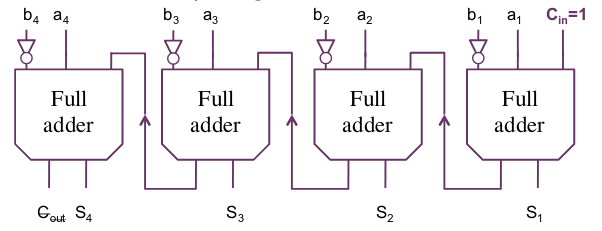
\includegraphics[scale=0.7]{Subtractor}
\end{center}
\subsection{Decoder}
If we want to activate a specific byte from a large amount of memory, this is how we do it. Giving the binary representation of the number as input the output will be the line corresponding to that number.
\begin{center}
	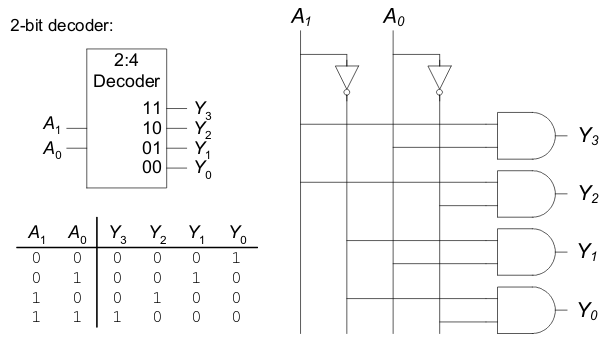
\includegraphics[scale=0.7]{Decoder}
\end{center}
\subsection{Multiplexor}
This has a selector which takes a binary input and outputs one of the $D$ inputs corresponding to that valie
\begin{center}
	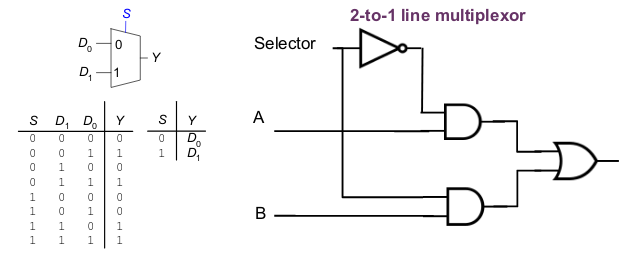
\includegraphics[scale=0.7]{Mux}
\end{center}
\subsection{Tristate}
\begin{center}
	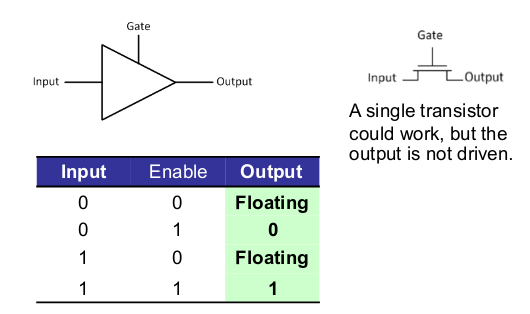
\includegraphics[scale=0.7]{Tristate}
\end{center}
There is also the inverting tristate, which has a wild circuit, but is just the tristate notted
\begin{center}
	\includegraphics[scale=0.7]{"Inverting Tristate"}
\end{center}
Muxes can be simplified using tristates, also note that muxes can be chained for simplicity
\begin{center}
	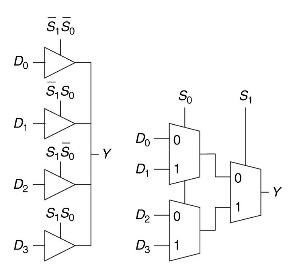
\includegraphics[scale=0.7]{Mux1}
\end{center}
\section{Timing and Advanced Adders}
Propagation delay ($t_{pd}$) - The max delay before the output is stable\\
Contamination delay ($t_{cd}$) - The min delay before the input changes\\
\\
Delay is caused by:
\begin{itemize}
	\item Capacitance and resistance in a circuit
	\item The speed of light limitation
\end{itemize}
Reasons why $t_{pd}$ and $t_{cd}$ may be different
\begin{itemize}
	\item Different rising and falling delays
	\item A circuit may have multiple inputs and outputs, some of which are faster than others
	\item Circuit speed with relation to temperature
\end{itemize}
\subsection{Critical paths}
\textbf{Critical path} - The longest path in the circuit - this determines the propagation delay\\
\textbf{Short path} - The shortest path in the circuit - this determines the contamination delay
\subsection{Glitches}
\textbf{Glitch} - Where an output will temporarily move to an incorrect value before stabilising
\subsection{Carry Lookahead Adders}
Define two functions:
\textbf{Generate}: G(A,B)=1 if A and B could cause $C_{out}$ even if $C_{in}=0$ (A AND B)\\
\textbf{Propagate}: P(A,B)=1 if A and B would cause $C_{out}$ if $C_{in}=1$ (A or B)\\
\\
This allows carry out to be calculated as
\[
\mathrm{C}_{\mathrm{out}}=\mathrm{G}(\mathrm{A}, \mathrm{B})+\mathrm{P}(\mathrm{A}, \mathrm{B}) \cdot \mathrm{C}_{\mathrm{in}}
\]
When expanding to larger numbers of bits, it is better to chain smaller CLAs to save gates
\section{Sequential Circuits}
\begin{itemize}
	\item Output depends on history as well as current input (i.e. the circuit has memory)
	\item Can be modelled as Finite State Machines
	\item Fundamental components of latches and flip flops
\end{itemize}
Synchronous sequential circuits - Made from combinatorial components interleaved with banks of flip flops containing the state of the circuit
\subsection{SR-Latch}
Also known as a NOR latch
\begin{center}
	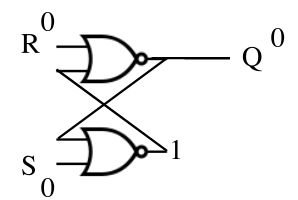
\includegraphics[scale=0.7]{SR-Latch}
\end{center}
\begin{itemize}
	\item Both inputs "usually" set to 0
	\item If input S (set) has a pulse of 1, the output becomes 1
	\item The output remains 1 even when the pulse is over
	\item If input R (reset) has a pulse of 1, the output becomes 0
	\item The output remains 0 even when the pulse is over
	\item If the output is already 1, a pulse on S will not change it. If it is already 0, a pulse on R will not change it
	\item It is called \textbf{bistable} as it has two stable states for a given input
\end{itemize}
This gate can also be built from AND gates, but the usual states are 1 rather than 0
\subsection{D-Latch}
In a latch a pulse on set or reset indicates what the new state should be, and when it should change
\begin{center}
	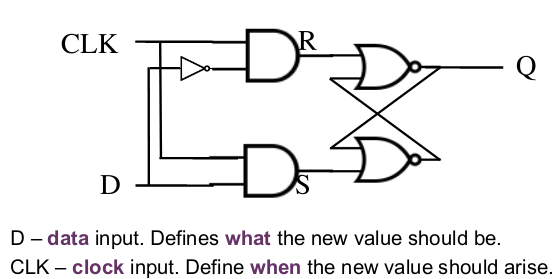
\includegraphics[scale=0.7]{D-latch}
\end{center}
\subsection{D Flip-Flop}
Instead of the output changing \textbf{whenever} the clock is high, the D Flip-Flop changes \textbf{only at the moment the clock goes high}
\begin{center}
	\includegraphics[scale=0.7]{"D Flip-Flop"}
\end{center}
These can be combined to form a register.\\
\textbf{Register} - A bank of flip-flops driven by the same clock
\begin{center}
	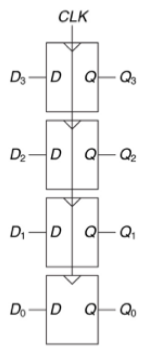
\includegraphics[scale=0.7]{Register}
\end{center}
\subsection{Enabled Flip-Flop}
This has an additional input (enable) to control whether the data is loaded into the register or not
\begin{center}
	\includegraphics[scale=0.7]{"Enabled Flip-Flop"}
\end{center}
\textbf{Gated Clock} - Where there is a gate to control if the clock gets to the flip flop.\\
There can be timing errors and glitches with Gated Clocks
\subsection{Problem Circuits}
A Unstable/Astable circuit can be seen below
\begin{center}
	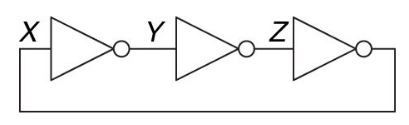
\includegraphics[scale=0.7]{Unstable}
\end{center}
\textbf{Race condition} - Behaviour depends on which two routes through the circuits carry the signal the fastest\\
\\
\textbf{Loops/Cyclic Paths} - Where outputs are fed back into inputs\\
To avoid this we insert registers into cyclic paths:
\begin{itemize}
	\item The registers contain the 'state' of the circuit
	\item They break the paths
	\item They only update on a clock edge
	\item Say they are synchronised to the clock
\end{itemize}
\subsection{Synchronous Circuits}
A synchronous sequential circuit consists of interconnected elements such that:
\begin{itemize}
	\item Every circuit is either a register or combinational circuit
	\item At least one circuit element is a register
	\item All registers receive the same clock signal
	\item Every cyclic path contains at least one register
\end{itemize}
A synchronous sequential circuit has:
\begin{itemize}
	\item A discrete set of states $\{S_0,...,S_{k-1}\}$
	\item A clock input, whose rising edge indicates when a state change occurs
	\item A functional specification which details the next state and all outputs for each possible current state and set of inputs
\end{itemize}
\subsection{Timing}
\begin{itemize}
	\item $t_{setup}$ - Time before rising edge during which inputs must be stable
	\item $t_{hold}$ - Time after rising edge during which inputs must be stable
	\item $t_{ccq}$ - Time until output starts to change
	\item $t_{pcq}$ - Time by which output has stabilized
\end{itemize}
\begin{center}
	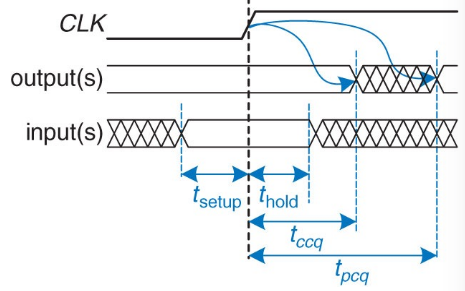
\includegraphics[scale=0.7]{Timing}
\end{center}
\subsection{Setting Time}
Time between ticks ($T_c$) must be at least $t_{pcq}+t_{pd}+t_{setup}$\\
\textbf{Sequencing Overhead} - $t_{pcq}+t_{setup}$\\
\\
There is also a minimum delay requirement
After the clock change, there is a time of $t_{ccq}+t_{cd}$ before the output starts changing, so $t_{hold}$ needs to be at least this
\subsection{Metastable states}
\textbf{Metastable state} - A state that will be driven to 1 or 0 eventually, but may take time
\subsection{Synchronisers}
A pair of flip flops can be used to synchronise the input with the clock
\section{Memory}
3 Common Types:
\begin{itemize}
	\item Dynamic Random Access Memory
	\item Static Random Access Memory
	\item Read Only Memory (ROM)
\end{itemize}
Memory is constructed with N address bits and M data bits
\begin{itemize}
	\item $2^N$ rows and $M$ data bits
	\item Depth: Number of rows (number of words)]
	\item Width: Number of columns (size of word)
	\item Array Size: depth $\times$ width = $2^N\times M$
\end{itemize}
Wordline:
\begin{itemize}
	\item Single row in a memory array to be read/written
	\item Only one wordline is HIGH at once
\end{itemize}
On memory read:
\begin{itemize}
	\item If the wordline is active (high) the stored but should drive the bitline value
	\item If the wordline is not active (low) the stored bit should not affect the bitline
\end{itemize}
Memory consists of latches, each holding a single bit value, at an address\\
\\
MAR holds the 'open' address\\
MDR holds the activated data
\subsection{Lines}
\textbf{Wordline/Address Line} - On when computer is addressing the data in that cell\\
\textbf{Read/Write Line} - Determines whether the data will be transferred to the MDR (write) or from the MDR(read) from the cell\\
\\
\textbf{Read} occurs when:
\begin{itemize}
	\item Address Line=1 AND R/W line=1
\end{itemize}
\textbf{Write occurs when}:
\begin{itemize}
	\item Address line=1 AND R/W line=0
\end{itemize}
\subsection{DRAM}
Each bit is one transistor and one capacitor\\
Need refreshing as capacitors discharge
\subsection{SRAM}
6 (or more) transistor flip-flop based memory\\
Low density but stable and fast
\subsection{ROM}
In a similar way to DRAM, but replace capacitor with connection to ground or high\\
PROM (Programmable ROM) works in a similar way, but has fuses connecting each transistor to high, these can be blown to create the data
\subsection{Memory Interleaving}
Basically RAID 0
\subsection{Cache hit and miss}
\textbf{Cache miss} - Look something up in memory and it is not found\\
\textbf{Cache hit} - Look something up in memory and it is found.
\section{Addressing Modes}
Sometimes we would like to
\begin{itemize}
	\item Address a large amount of memory with only a few bits
	\item Use indexes to loop or examine a table or array
	\item Relocate data or programs in the memory
	\item Operate on the registers rather than the actual memory
\end{itemize}
This can be achieved using alternate addressing modes
\begin{itemize}
	\item Direct addressing - The address read in the instruction is the address of the actual data
	\item Immediate addressing - The address read in the instruction is the data to be used
	\item Indirect addressing - The address read in the instruction is the address of a memory location containing the address of the actual data
	\item Register indirect addressing - The address read in the instruction is the address of a register containing the address of the actual data
	\item Indexed addressing - The address read in the instruction should have an index value (contained in some register) added to obtain the address of the data
\end{itemize}
Alternative to absolute addressing
\begin{itemize}
	\item Absolute Addressing - The address is the one containing the data
	\item Relative addressing - The address is an offset to the current instruction address
	\item Base offset addressing - The address read is offset by the current value in a special 'base' register
\end{itemize}
\section{Microarchitecture}
\textbf{Architecture} - Consists of instruction set and implies an architectural state\\
\textbf{Microarchitecture} - How to implement an architecture in hardware, made of
\begin{itemize}
	\item Datapath - functional blocks and registers
	\item Control - Control signals
\end{itemize}
\end{document}
